% Created by tikzDevice version 0.6.2-92-0ad2792 on 2013-03-23 23:05:17
% !TEX encoding = UTF-8 Unicode
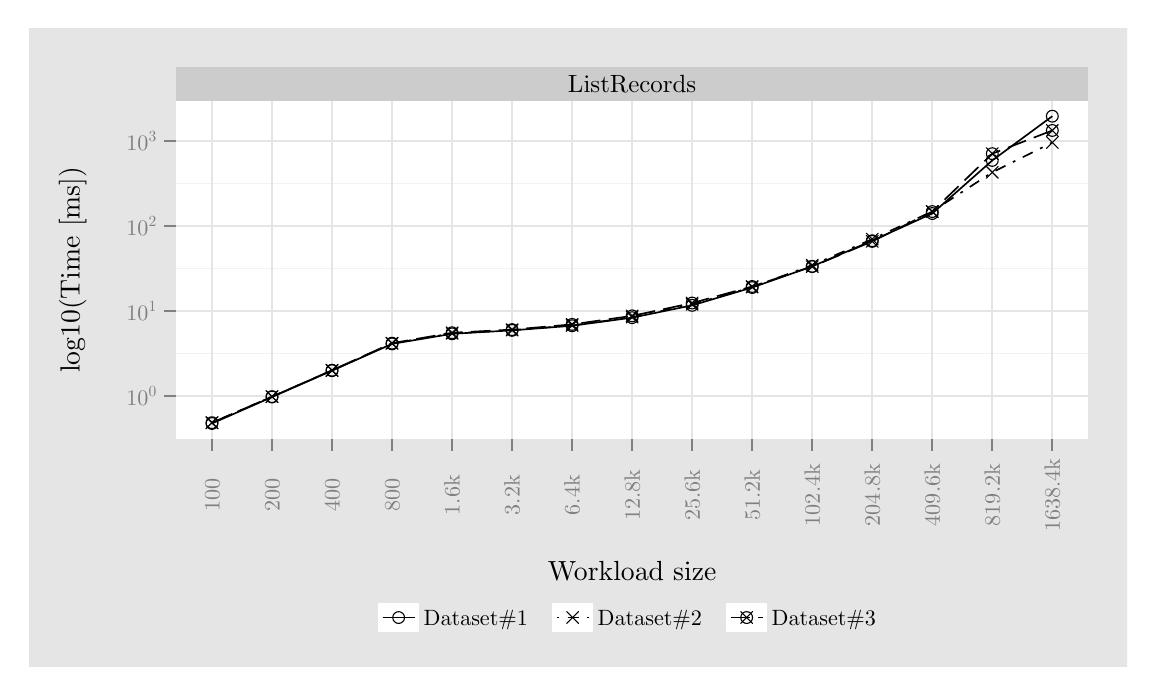
\begin{tikzpicture}[x=1pt,y=1pt]
\definecolor[named]{fillColor}{rgb}{1.00,1.00,1.00}
\path[use as bounding box,fill=fillColor,fill opacity=0.00] (0,0) rectangle (397.48,231.26);
\begin{scope}
\path[clip] (  0.00,  0.00) rectangle (397.48,231.26);
\definecolor[named]{drawColor}{rgb}{1.00,1.00,1.00}
\definecolor[named]{fillColor}{rgb}{0.90,0.90,0.90}

\path[draw=drawColor,line width= 0.6pt,line join=round,line cap=round,fill=fillColor] (  0.00,  0.00) rectangle (397.48,231.26);
\end{scope}
\begin{scope}
\path[clip] ( 53.58, 82.69) rectangle (383.26,204.82);
\definecolor[named]{fillColor}{rgb}{1.00,1.00,1.00}

\path[fill=fillColor] ( 53.58, 82.69) rectangle (383.26,204.82);
\definecolor[named]{drawColor}{rgb}{0.95,0.95,0.95}

\path[draw=drawColor,line width= 0.3pt,line join=round] ( 53.58,113.45) --
	(383.26,113.45);

\path[draw=drawColor,line width= 0.3pt,line join=round] ( 53.58,144.24) --
	(383.26,144.24);

\path[draw=drawColor,line width= 0.3pt,line join=round] ( 53.58,175.03) --
	(383.26,175.03);
\definecolor[named]{drawColor}{rgb}{0.90,0.90,0.90}

\path[draw=drawColor,line width= 0.6pt,line join=round] ( 53.58, 98.06) --
	(383.26, 98.06);

\path[draw=drawColor,line width= 0.6pt,line join=round] ( 53.58,128.85) --
	(383.26,128.85);

\path[draw=drawColor,line width= 0.6pt,line join=round] ( 53.58,159.64) --
	(383.26,159.64);

\path[draw=drawColor,line width= 0.6pt,line join=round] ( 53.58,190.42) --
	(383.26,190.42);

\path[draw=drawColor,line width= 0.6pt,line join=round] ( 66.60, 82.69) --
	( 66.60,204.82);

\path[draw=drawColor,line width= 0.6pt,line join=round] ( 88.29, 82.69) --
	( 88.29,204.82);

\path[draw=drawColor,line width= 0.6pt,line join=round] (109.97, 82.69) --
	(109.97,204.82);

\path[draw=drawColor,line width= 0.6pt,line join=round] (131.66, 82.69) --
	(131.66,204.82);

\path[draw=drawColor,line width= 0.6pt,line join=round] (153.35, 82.69) --
	(153.35,204.82);

\path[draw=drawColor,line width= 0.6pt,line join=round] (175.04, 82.69) --
	(175.04,204.82);

\path[draw=drawColor,line width= 0.6pt,line join=round] (196.73, 82.69) --
	(196.73,204.82);

\path[draw=drawColor,line width= 0.6pt,line join=round] (218.42, 82.69) --
	(218.42,204.82);

\path[draw=drawColor,line width= 0.6pt,line join=round] (240.11, 82.69) --
	(240.11,204.82);

\path[draw=drawColor,line width= 0.6pt,line join=round] (261.80, 82.69) --
	(261.80,204.82);

\path[draw=drawColor,line width= 0.6pt,line join=round] (283.49, 82.69) --
	(283.49,204.82);

\path[draw=drawColor,line width= 0.6pt,line join=round] (305.18, 82.69) --
	(305.18,204.82);

\path[draw=drawColor,line width= 0.6pt,line join=round] (326.87, 82.69) --
	(326.87,204.82);

\path[draw=drawColor,line width= 0.6pt,line join=round] (348.56, 82.69) --
	(348.56,204.82);

\path[draw=drawColor,line width= 0.6pt,line join=round] (370.25, 82.69) --
	(370.25,204.82);
\definecolor[named]{drawColor}{rgb}{0.00,0.00,0.00}

\path[draw=drawColor,line width= 0.6pt,line join=round] ( 66.60, 88.24) --
	( 88.29, 97.79) --
	(109.97,107.32) --
	(131.66,116.99) --
	(153.35,120.63) --
	(175.04,121.88) --
	(196.73,123.55) --
	(218.42,126.47) --
	(240.11,130.92) --
	(261.80,137.36) --
	(283.49,145.00) --
	(305.18,154.27) --
	(326.87,164.11) --
	(348.56,183.29) --
	(370.25,199.27);

\path[draw=drawColor,line width= 0.6pt,dash pattern=on 1pt off 3pt on 4pt off 3pt ,line join=round] ( 66.60, 88.52) --
	( 88.29, 97.92) --
	(109.97,107.39) --
	(131.66,117.15) --
	(153.35,120.78) --
	(175.04,121.95) --
	(196.73,123.65) --
	(218.42,126.66) --
	(240.11,131.25) --
	(261.80,137.50) --
	(283.49,145.46) --
	(305.18,154.83) --
	(326.87,164.86) --
	(348.56,179.00) --
	(370.25,189.76);

\path[draw=drawColor,line width= 0.6pt,dash pattern=on 7pt off 3pt ,line join=round] ( 66.60, 88.52) --
	( 88.29, 97.92) --
	(109.97,107.46) --
	(131.66,117.25) --
	(153.35,121.02) --
	(175.04,122.15) --
	(196.73,124.04) --
	(218.42,127.12) --
	(240.11,131.75) --
	(261.80,137.73) --
	(283.49,144.94) --
	(305.18,154.03) --
	(326.87,164.81) --
	(348.56,185.73) --
	(370.25,194.11);

\path[draw=drawColor,line width= 0.4pt,line join=round,line cap=round] ( 66.60, 88.24) circle (  2.13);

\path[draw=drawColor,line width= 0.4pt,line join=round,line cap=round] ( 88.29, 97.79) circle (  2.13);

\path[draw=drawColor,line width= 0.4pt,line join=round,line cap=round] (109.97,107.32) circle (  2.13);

\path[draw=drawColor,line width= 0.4pt,line join=round,line cap=round] (131.66,116.99) circle (  2.13);

\path[draw=drawColor,line width= 0.4pt,line join=round,line cap=round] (153.35,120.63) circle (  2.13);

\path[draw=drawColor,line width= 0.4pt,line join=round,line cap=round] (175.04,121.88) circle (  2.13);

\path[draw=drawColor,line width= 0.4pt,line join=round,line cap=round] (196.73,123.55) circle (  2.13);

\path[draw=drawColor,line width= 0.4pt,line join=round,line cap=round] (218.42,126.47) circle (  2.13);

\path[draw=drawColor,line width= 0.4pt,line join=round,line cap=round] (240.11,130.92) circle (  2.13);

\path[draw=drawColor,line width= 0.4pt,line join=round,line cap=round] (261.80,137.36) circle (  2.13);

\path[draw=drawColor,line width= 0.4pt,line join=round,line cap=round] (283.49,145.00) circle (  2.13);

\path[draw=drawColor,line width= 0.4pt,line join=round,line cap=round] (305.18,154.27) circle (  2.13);

\path[draw=drawColor,line width= 0.4pt,line join=round,line cap=round] (326.87,164.11) circle (  2.13);

\path[draw=drawColor,line width= 0.4pt,line join=round,line cap=round] (348.56,183.29) circle (  2.13);

\path[draw=drawColor,line width= 0.4pt,line join=round,line cap=round] (370.25,199.27) circle (  2.13);

\path[draw=drawColor,line width= 0.4pt,line join=round,line cap=round] ( 66.60, 88.52) circle (  2.13);

\path[draw=drawColor,line width= 0.4pt,line join=round,line cap=round] ( 64.46, 86.38) -- ( 68.73, 90.65);

\path[draw=drawColor,line width= 0.4pt,line join=round,line cap=round] ( 64.46, 90.65) -- ( 68.73, 86.38);

\path[draw=drawColor,line width= 0.4pt,line join=round,line cap=round] ( 88.29, 97.92) circle (  2.13);

\path[draw=drawColor,line width= 0.4pt,line join=round,line cap=round] ( 86.15, 95.79) -- ( 90.42,100.06);

\path[draw=drawColor,line width= 0.4pt,line join=round,line cap=round] ( 86.15,100.06) -- ( 90.42, 95.79);

\path[draw=drawColor,line width= 0.4pt,line join=round,line cap=round] (109.97,107.46) circle (  2.13);

\path[draw=drawColor,line width= 0.4pt,line join=round,line cap=round] (107.84,105.32) -- (112.11,109.59);

\path[draw=drawColor,line width= 0.4pt,line join=round,line cap=round] (107.84,109.59) -- (112.11,105.32);

\path[draw=drawColor,line width= 0.4pt,line join=round,line cap=round] (131.66,117.25) circle (  2.13);

\path[draw=drawColor,line width= 0.4pt,line join=round,line cap=round] (129.53,115.11) -- (133.80,119.38);

\path[draw=drawColor,line width= 0.4pt,line join=round,line cap=round] (129.53,119.38) -- (133.80,115.11);

\path[draw=drawColor,line width= 0.4pt,line join=round,line cap=round] (153.35,121.02) circle (  2.13);

\path[draw=drawColor,line width= 0.4pt,line join=round,line cap=round] (151.22,118.89) -- (155.49,123.15);

\path[draw=drawColor,line width= 0.4pt,line join=round,line cap=round] (151.22,123.15) -- (155.49,118.89);

\path[draw=drawColor,line width= 0.4pt,line join=round,line cap=round] (175.04,122.15) circle (  2.13);

\path[draw=drawColor,line width= 0.4pt,line join=round,line cap=round] (172.91,120.01) -- (177.18,124.28);

\path[draw=drawColor,line width= 0.4pt,line join=round,line cap=round] (172.91,124.28) -- (177.18,120.01);

\path[draw=drawColor,line width= 0.4pt,line join=round,line cap=round] (196.73,124.04) circle (  2.13);

\path[draw=drawColor,line width= 0.4pt,line join=round,line cap=round] (194.60,121.90) -- (198.87,126.17);

\path[draw=drawColor,line width= 0.4pt,line join=round,line cap=round] (194.60,126.17) -- (198.87,121.90);

\path[draw=drawColor,line width= 0.4pt,line join=round,line cap=round] (218.42,127.12) circle (  2.13);

\path[draw=drawColor,line width= 0.4pt,line join=round,line cap=round] (216.29,124.99) -- (220.55,129.26);

\path[draw=drawColor,line width= 0.4pt,line join=round,line cap=round] (216.29,129.26) -- (220.55,124.99);

\path[draw=drawColor,line width= 0.4pt,line join=round,line cap=round] (240.11,131.75) circle (  2.13);

\path[draw=drawColor,line width= 0.4pt,line join=round,line cap=round] (237.98,129.62) -- (242.24,133.89);

\path[draw=drawColor,line width= 0.4pt,line join=round,line cap=round] (237.98,133.89) -- (242.24,129.62);

\path[draw=drawColor,line width= 0.4pt,line join=round,line cap=round] (261.80,137.73) circle (  2.13);

\path[draw=drawColor,line width= 0.4pt,line join=round,line cap=round] (259.67,135.59) -- (263.93,139.86);

\path[draw=drawColor,line width= 0.4pt,line join=round,line cap=round] (259.67,139.86) -- (263.93,135.59);

\path[draw=drawColor,line width= 0.4pt,line join=round,line cap=round] (283.49,144.94) circle (  2.13);

\path[draw=drawColor,line width= 0.4pt,line join=round,line cap=round] (281.35,142.80) -- (285.62,147.07);

\path[draw=drawColor,line width= 0.4pt,line join=round,line cap=round] (281.35,147.07) -- (285.62,142.80);

\path[draw=drawColor,line width= 0.4pt,line join=round,line cap=round] (305.18,154.03) circle (  2.13);

\path[draw=drawColor,line width= 0.4pt,line join=round,line cap=round] (303.04,151.90) -- (307.31,156.17);

\path[draw=drawColor,line width= 0.4pt,line join=round,line cap=round] (303.04,156.17) -- (307.31,151.90);

\path[draw=drawColor,line width= 0.4pt,line join=round,line cap=round] (326.87,164.81) circle (  2.13);

\path[draw=drawColor,line width= 0.4pt,line join=round,line cap=round] (324.73,162.67) -- (329.00,166.94);

\path[draw=drawColor,line width= 0.4pt,line join=round,line cap=round] (324.73,166.94) -- (329.00,162.67);

\path[draw=drawColor,line width= 0.4pt,line join=round,line cap=round] (348.56,185.73) circle (  2.13);

\path[draw=drawColor,line width= 0.4pt,line join=round,line cap=round] (346.42,183.60) -- (350.69,187.87);

\path[draw=drawColor,line width= 0.4pt,line join=round,line cap=round] (346.42,187.87) -- (350.69,183.60);

\path[draw=drawColor,line width= 0.4pt,line join=round,line cap=round] (370.25,194.11) circle (  2.13);

\path[draw=drawColor,line width= 0.4pt,line join=round,line cap=round] (368.11,191.98) -- (372.38,196.25);

\path[draw=drawColor,line width= 0.4pt,line join=round,line cap=round] (368.11,196.25) -- (372.38,191.98);

\path[draw=drawColor,line width= 0.4pt,line join=round,line cap=round,fill=fillColor] ( 64.46, 86.38) -- ( 68.73, 90.65);

\path[draw=drawColor,line width= 0.4pt,line join=round,line cap=round,fill=fillColor] ( 64.46, 90.65) -- ( 68.73, 86.38);

\path[draw=drawColor,line width= 0.4pt,line join=round,line cap=round,fill=fillColor] ( 86.15, 95.79) -- ( 90.42,100.06);

\path[draw=drawColor,line width= 0.4pt,line join=round,line cap=round,fill=fillColor] ( 86.15,100.06) -- ( 90.42, 95.79);

\path[draw=drawColor,line width= 0.4pt,line join=round,line cap=round,fill=fillColor] (107.84,105.26) -- (112.11,109.53);

\path[draw=drawColor,line width= 0.4pt,line join=round,line cap=round,fill=fillColor] (107.84,109.53) -- (112.11,105.26);

\path[draw=drawColor,line width= 0.4pt,line join=round,line cap=round,fill=fillColor] (129.53,115.02) -- (133.80,119.28);

\path[draw=drawColor,line width= 0.4pt,line join=round,line cap=round,fill=fillColor] (129.53,119.28) -- (133.80,115.02);

\path[draw=drawColor,line width= 0.4pt,line join=round,line cap=round,fill=fillColor] (151.22,118.64) -- (155.49,122.91);

\path[draw=drawColor,line width= 0.4pt,line join=round,line cap=round,fill=fillColor] (151.22,122.91) -- (155.49,118.64);

\path[draw=drawColor,line width= 0.4pt,line join=round,line cap=round,fill=fillColor] (172.91,119.81) -- (177.18,124.08);

\path[draw=drawColor,line width= 0.4pt,line join=round,line cap=round,fill=fillColor] (172.91,124.08) -- (177.18,119.81);

\path[draw=drawColor,line width= 0.4pt,line join=round,line cap=round,fill=fillColor] (194.60,121.52) -- (198.87,125.78);

\path[draw=drawColor,line width= 0.4pt,line join=round,line cap=round,fill=fillColor] (194.60,125.78) -- (198.87,121.52);

\path[draw=drawColor,line width= 0.4pt,line join=round,line cap=round,fill=fillColor] (216.29,124.52) -- (220.55,128.79);

\path[draw=drawColor,line width= 0.4pt,line join=round,line cap=round,fill=fillColor] (216.29,128.79) -- (220.55,124.52);

\path[draw=drawColor,line width= 0.4pt,line join=round,line cap=round,fill=fillColor] (237.98,129.12) -- (242.24,133.38);

\path[draw=drawColor,line width= 0.4pt,line join=round,line cap=round,fill=fillColor] (237.98,133.38) -- (242.24,129.12);

\path[draw=drawColor,line width= 0.4pt,line join=round,line cap=round,fill=fillColor] (259.67,135.36) -- (263.93,139.63);

\path[draw=drawColor,line width= 0.4pt,line join=round,line cap=round,fill=fillColor] (259.67,139.63) -- (263.93,135.36);

\path[draw=drawColor,line width= 0.4pt,line join=round,line cap=round,fill=fillColor] (281.35,143.32) -- (285.62,147.59);

\path[draw=drawColor,line width= 0.4pt,line join=round,line cap=round,fill=fillColor] (281.35,147.59) -- (285.62,143.32);

\path[draw=drawColor,line width= 0.4pt,line join=round,line cap=round,fill=fillColor] (303.04,152.70) -- (307.31,156.97);

\path[draw=drawColor,line width= 0.4pt,line join=round,line cap=round,fill=fillColor] (303.04,156.97) -- (307.31,152.70);

\path[draw=drawColor,line width= 0.4pt,line join=round,line cap=round,fill=fillColor] (324.73,162.73) -- (329.00,167.00);

\path[draw=drawColor,line width= 0.4pt,line join=round,line cap=round,fill=fillColor] (324.73,167.00) -- (329.00,162.73);

\path[draw=drawColor,line width= 0.4pt,line join=round,line cap=round,fill=fillColor] (346.42,176.87) -- (350.69,181.13);

\path[draw=drawColor,line width= 0.4pt,line join=round,line cap=round,fill=fillColor] (346.42,181.13) -- (350.69,176.87);

\path[draw=drawColor,line width= 0.4pt,line join=round,line cap=round,fill=fillColor] (368.11,187.63) -- (372.38,191.90);

\path[draw=drawColor,line width= 0.4pt,line join=round,line cap=round,fill=fillColor] (368.11,191.90) -- (372.38,187.63);
\end{scope}
\begin{scope}
\path[clip] (  0.00,  0.00) rectangle (397.48,231.26);
\definecolor[named]{fillColor}{rgb}{0.80,0.80,0.80}

\path[fill=fillColor] ( 53.58,204.82) rectangle (383.26,217.04);
\definecolor[named]{drawColor}{rgb}{0.00,0.00,0.00}

\node[text=drawColor,anchor=base,inner sep=0pt, outer sep=0pt, scale=  0.90] at (218.42,207.83) {ListRecords};
\end{scope}
\begin{scope}
\path[clip] (  0.00,  0.00) rectangle (397.48,231.26);
\definecolor[named]{drawColor}{rgb}{0.50,0.50,0.50}

\node[text=drawColor,anchor=base west,inner sep=0pt, outer sep=0pt, scale=  0.80] at ( 35.67, 94.62) {10};

\node[text=drawColor,anchor=base west,inner sep=0pt, outer sep=0pt, scale=  0.56] at ( 43.67, 97.90) {0};

\node[text=drawColor,anchor=base west,inner sep=0pt, outer sep=0pt, scale=  0.80] at ( 35.67,125.41) {10};

\node[text=drawColor,anchor=base west,inner sep=0pt, outer sep=0pt, scale=  0.56] at ( 43.67,128.69) {1};

\node[text=drawColor,anchor=base west,inner sep=0pt, outer sep=0pt, scale=  0.80] at ( 35.67,156.20) {10};

\node[text=drawColor,anchor=base west,inner sep=0pt, outer sep=0pt, scale=  0.56] at ( 43.67,159.47) {2};

\node[text=drawColor,anchor=base west,inner sep=0pt, outer sep=0pt, scale=  0.80] at ( 35.67,186.99) {10};

\node[text=drawColor,anchor=base west,inner sep=0pt, outer sep=0pt, scale=  0.56] at ( 43.67,190.26) {3};
\end{scope}
\begin{scope}
\path[clip] (  0.00,  0.00) rectangle (397.48,231.26);
\definecolor[named]{drawColor}{rgb}{0.50,0.50,0.50}

\path[draw=drawColor,line width= 0.6pt,line join=round] ( 49.31, 98.06) --
	( 53.58, 98.06);

\path[draw=drawColor,line width= 0.6pt,line join=round] ( 49.31,128.85) --
	( 53.58,128.85);

\path[draw=drawColor,line width= 0.6pt,line join=round] ( 49.31,159.64) --
	( 53.58,159.64);

\path[draw=drawColor,line width= 0.6pt,line join=round] ( 49.31,190.42) --
	( 53.58,190.42);
\end{scope}
\begin{scope}
\path[clip] (  0.00,  0.00) rectangle (397.48,231.26);
\definecolor[named]{drawColor}{rgb}{0.50,0.50,0.50}

\path[draw=drawColor,line width= 0.6pt,line join=round] ( 66.60, 78.42) --
	( 66.60, 82.69);

\path[draw=drawColor,line width= 0.6pt,line join=round] ( 88.29, 78.42) --
	( 88.29, 82.69);

\path[draw=drawColor,line width= 0.6pt,line join=round] (109.97, 78.42) --
	(109.97, 82.69);

\path[draw=drawColor,line width= 0.6pt,line join=round] (131.66, 78.42) --
	(131.66, 82.69);

\path[draw=drawColor,line width= 0.6pt,line join=round] (153.35, 78.42) --
	(153.35, 82.69);

\path[draw=drawColor,line width= 0.6pt,line join=round] (175.04, 78.42) --
	(175.04, 82.69);

\path[draw=drawColor,line width= 0.6pt,line join=round] (196.73, 78.42) --
	(196.73, 82.69);

\path[draw=drawColor,line width= 0.6pt,line join=round] (218.42, 78.42) --
	(218.42, 82.69);

\path[draw=drawColor,line width= 0.6pt,line join=round] (240.11, 78.42) --
	(240.11, 82.69);

\path[draw=drawColor,line width= 0.6pt,line join=round] (261.80, 78.42) --
	(261.80, 82.69);

\path[draw=drawColor,line width= 0.6pt,line join=round] (283.49, 78.42) --
	(283.49, 82.69);

\path[draw=drawColor,line width= 0.6pt,line join=round] (305.18, 78.42) --
	(305.18, 82.69);

\path[draw=drawColor,line width= 0.6pt,line join=round] (326.87, 78.42) --
	(326.87, 82.69);

\path[draw=drawColor,line width= 0.6pt,line join=round] (348.56, 78.42) --
	(348.56, 82.69);

\path[draw=drawColor,line width= 0.6pt,line join=round] (370.25, 78.42) --
	(370.25, 82.69);
\end{scope}
\begin{scope}
\path[clip] (  0.00,  0.00) rectangle (397.48,231.26);
\definecolor[named]{drawColor}{rgb}{0.50,0.50,0.50}

\node[text=drawColor,rotate= 90.00,anchor=base,inner sep=0pt, outer sep=0pt, scale=  0.80] at ( 69.35, 62.36) {100};

\node[text=drawColor,rotate= 90.00,anchor=base,inner sep=0pt, outer sep=0pt, scale=  0.80] at ( 91.04, 62.36) {200};

\node[text=drawColor,rotate= 90.00,anchor=base,inner sep=0pt, outer sep=0pt, scale=  0.80] at (112.73, 62.36) {400};

\node[text=drawColor,rotate= 90.00,anchor=base,inner sep=0pt, outer sep=0pt, scale=  0.80] at (134.42, 62.36) {800};

\node[text=drawColor,rotate= 90.00,anchor=base,inner sep=0pt, outer sep=0pt, scale=  0.80] at (156.11, 62.36) {1.6k};

\node[text=drawColor,rotate= 90.00,anchor=base,inner sep=0pt, outer sep=0pt, scale=  0.80] at (177.80, 62.36) {3.2k};

\node[text=drawColor,rotate= 90.00,anchor=base,inner sep=0pt, outer sep=0pt, scale=  0.80] at (199.49, 62.36) {6.4k};

\node[text=drawColor,rotate= 90.00,anchor=base,inner sep=0pt, outer sep=0pt, scale=  0.80] at (221.18, 62.36) {12.8k};

\node[text=drawColor,rotate= 90.00,anchor=base,inner sep=0pt, outer sep=0pt, scale=  0.80] at (242.86, 62.36) {25.6k};

\node[text=drawColor,rotate= 90.00,anchor=base,inner sep=0pt, outer sep=0pt, scale=  0.80] at (264.55, 62.36) {51.2k};

\node[text=drawColor,rotate= 90.00,anchor=base,inner sep=0pt, outer sep=0pt, scale=  0.80] at (286.24, 62.36) {102.4k};

\node[text=drawColor,rotate= 90.00,anchor=base,inner sep=0pt, outer sep=0pt, scale=  0.80] at (307.93, 62.36) {204.8k};

\node[text=drawColor,rotate= 90.00,anchor=base,inner sep=0pt, outer sep=0pt, scale=  0.80] at (329.62, 62.36) {409.6k};

\node[text=drawColor,rotate= 90.00,anchor=base,inner sep=0pt, outer sep=0pt, scale=  0.80] at (351.31, 62.36) {819.2k};

\node[text=drawColor,rotate= 90.00,anchor=base,inner sep=0pt, outer sep=0pt, scale=  0.80] at (373.00, 62.36) {1638.4k};
\end{scope}
\begin{scope}
\path[clip] (  0.00,  0.00) rectangle (397.48,231.26);
\definecolor[named]{drawColor}{rgb}{0.00,0.00,0.00}

\node[text=drawColor,anchor=base,inner sep=0pt, outer sep=0pt, scale=  1.00] at (218.42, 31.41) {Workload size};
\end{scope}
\begin{scope}
\path[clip] (  0.00,  0.00) rectangle (397.48,231.26);
\definecolor[named]{drawColor}{rgb}{0.00,0.00,0.00}

\node[text=drawColor,rotate= 90.00,anchor=base,inner sep=0pt, outer sep=0pt, scale=  1.00] at ( 18.80,143.75) {log10(Time [ms])};
\end{scope}
\begin{scope}
\path[clip] (  0.00,  0.00) rectangle (397.48,231.26);
\definecolor[named]{fillColor}{rgb}{0.90,0.90,0.90}

\path[fill=fillColor] (118.93,  8.87) rectangle (317.91, 27.36);
\end{scope}
\begin{scope}
\path[clip] (  0.00,  0.00) rectangle (397.48,231.26);
\definecolor[named]{drawColor}{rgb}{1.00,1.00,1.00}
\definecolor[named]{fillColor}{rgb}{1.00,1.00,1.00}

\path[draw=drawColor,line width= 0.6pt,line join=round,line cap=round,fill=fillColor] (126.81, 13.14) rectangle (141.26, 23.09);
\end{scope}
\begin{scope}
\path[clip] (  0.00,  0.00) rectangle (397.48,231.26);
\definecolor[named]{drawColor}{rgb}{0.00,0.00,0.00}

\path[draw=drawColor,line width= 0.6pt,line join=round] (128.26, 18.11) -- (139.82, 18.11);
\end{scope}
\begin{scope}
\path[clip] (  0.00,  0.00) rectangle (397.48,231.26);
\definecolor[named]{drawColor}{rgb}{0.00,0.00,0.00}

\path[draw=drawColor,line width= 0.4pt,line join=round,line cap=round] (134.04, 18.11) circle (  2.13);
\end{scope}
\begin{scope}
\path[clip] (  0.00,  0.00) rectangle (397.48,231.26);
\definecolor[named]{drawColor}{rgb}{1.00,1.00,1.00}
\definecolor[named]{fillColor}{rgb}{1.00,1.00,1.00}

\path[draw=drawColor,line width= 0.6pt,line join=round,line cap=round,fill=fillColor] (189.69, 13.14) rectangle (204.14, 23.09);
\end{scope}
\begin{scope}
\path[clip] (  0.00,  0.00) rectangle (397.48,231.26);
\definecolor[named]{drawColor}{rgb}{0.00,0.00,0.00}

\path[draw=drawColor,line width= 0.6pt,dash pattern=on 1pt off 3pt on 4pt off 3pt ,line join=round] (191.14, 18.11) -- (202.70, 18.11);
\end{scope}
\begin{scope}
\path[clip] (  0.00,  0.00) rectangle (397.48,231.26);
\definecolor[named]{drawColor}{rgb}{0.00,0.00,0.00}
\definecolor[named]{fillColor}{rgb}{1.00,1.00,1.00}

\path[draw=drawColor,line width= 0.4pt,line join=round,line cap=round,fill=fillColor] (194.78, 15.98) -- (199.05, 20.25);

\path[draw=drawColor,line width= 0.4pt,line join=round,line cap=round,fill=fillColor] (194.78, 20.25) -- (199.05, 15.98);
\end{scope}
\begin{scope}
\path[clip] (  0.00,  0.00) rectangle (397.48,231.26);
\definecolor[named]{drawColor}{rgb}{1.00,1.00,1.00}
\definecolor[named]{fillColor}{rgb}{1.00,1.00,1.00}

\path[draw=drawColor,line width= 0.6pt,line join=round,line cap=round,fill=fillColor] (252.57, 13.14) rectangle (267.02, 23.09);
\end{scope}
\begin{scope}
\path[clip] (  0.00,  0.00) rectangle (397.48,231.26);
\definecolor[named]{drawColor}{rgb}{0.00,0.00,0.00}

\path[draw=drawColor,line width= 0.6pt,dash pattern=on 7pt off 3pt ,line join=round] (254.02, 18.11) -- (265.58, 18.11);
\end{scope}
\begin{scope}
\path[clip] (  0.00,  0.00) rectangle (397.48,231.26);
\definecolor[named]{drawColor}{rgb}{0.00,0.00,0.00}

\path[draw=drawColor,line width= 0.4pt,line join=round,line cap=round] (259.80, 18.11) circle (  2.13);

\path[draw=drawColor,line width= 0.4pt,line join=round,line cap=round] (257.66, 15.98) -- (261.93, 20.25);

\path[draw=drawColor,line width= 0.4pt,line join=round,line cap=round] (257.66, 20.25) -- (261.93, 15.98);
\end{scope}
\begin{scope}
\path[clip] (  0.00,  0.00) rectangle (397.48,231.26);
\definecolor[named]{drawColor}{rgb}{0.00,0.00,0.00}

\node[text=drawColor,anchor=base west,inner sep=0pt, outer sep=0pt, scale=  0.80] at (143.07, 15.36) {Dataset\#1 $\;\;$};
\end{scope}
\begin{scope}
\path[clip] (  0.00,  0.00) rectangle (397.48,231.26);
\definecolor[named]{drawColor}{rgb}{0.00,0.00,0.00}

\node[text=drawColor,anchor=base west,inner sep=0pt, outer sep=0pt, scale=  0.80] at (205.95, 15.36) {Dataset\#2 $\;\;$};
\end{scope}
\begin{scope}
\path[clip] (  0.00,  0.00) rectangle (397.48,231.26);
\definecolor[named]{drawColor}{rgb}{0.00,0.00,0.00}

\node[text=drawColor,anchor=base west,inner sep=0pt, outer sep=0pt, scale=  0.80] at (268.83, 15.36) {Dataset\#3 $\;\;$};
\end{scope}
\end{tikzpicture}
